% This must be in the first 5 lines to tell arXiv to use pdfLaTeX, which is strongly recommended.
\pdfoutput=1
% In particular, the hyperref package requires pdfLaTeX in order to break URLs across lines.

\documentclass[11pt]{article}

% Change "review" to "final" to generate the final (sometimes called camera-ready) version.
% Change to "preprint" to generate a non-anonymous version with page numbers.
\usepackage[final]{acl}

% Standard package includes
\usepackage{times}
\usepackage{latexsym}
% \usepackage[pagebackref,breaklinks,colorlinks,citecolor=cvprblue]{hyperref}
\usepackage{multirow}
\usepackage{booktabs}
% For proper rendering and hyphenation of words containing Latin characters (including in bib files)
\usepackage[T1]{fontenc}
% For Vietnamese characters
% \usepackage[T5]{fontenc}
% See https://www.latex-project.org/help/documentation/encguide.pdf for other character sets

% This assumes your files are encoded as UTF8
\usepackage[utf8]{inputenc}

\usepackage{microtype}
\usepackage{graphicx}
\usepackage{subcaption}
\usepackage{amsmath}
\usepackage{cleveref}
\usepackage{tcolorbox}

\usepackage{amssymb}
\usepackage{xcolor}
\usepackage{pifont}
\definecolor{my_green}{RGB}{51,102,0}
\definecolor{my_red}{RGB}{204, 0, 0}
\newcommand{\cmark}{\textcolor{my_green}{\ding{51}}} % ✔
\newcommand{\xmark}{\textcolor{my_red}{\ding{55}}} % ✘
\newcommand{\lilei}[1]{\textcolor{violet}{\bf \small [#1 --lilei]}}
\newcommand{\lpk}[1]{\textcolor{blue}{\bf \small [#1 --lpk]}}

% This is also not strictly necessary, and may be commented out.
% However, it will improve the aesthetics of text in
% the typewriter font.
\usepackage{inconsolata}

% If the title and author information does not fit in the area allocated, uncomment the following
%
%\setlength\titlebox{<dim>}
%
% and set <dim> to something 5cm or larger.

\title{Multimodal ArXiv: A Dataset for Improving Scientific Comprehension of Large Vision-Language Models}

% Author information can be set in various styles:
% For several authors from the same institution:
% \author{Author 1 \and ... \and Author n \\
%         Address line \\ ... \\ Address line}
% if the names do not fit well on one line use
%         Author 1 \\ {\bf Author 2} \\ ... \\ {\bf Author n} \\
% For authors from different institutions:
% \author{Author 1 \\ Address line \\  ... \\ Address line
%         \And  ... \And
%         Author n \\ Address line \\ ... \\ Address line}
% To start a separate ``row'' of authors use \AND, as in
% \author{Author 1 \\ Address line \\  ... \\ Address line
%         \AND
%         Author 2 \\ Address line \\ ... \\ Address line \And
%         Author 3 \\ Address line \\ ... \\ Address line}

\author{
Lei Li\thanks{Equal Contribution.}$^\dagger$,  Yuqi Wang$^*$$^\dagger$, Runxin Xu$^\ddag$, Peiyi Wang$^\ddag$\\\textbf{Xiachong Feng$^\dagger$, Lingpeng Kong$^\dagger$, Qi Liu$^\dagger$}\\ 
$^\dagger$The University of Hong Kong \\
$^\ddagger$Peking University\\
 \texttt{\{nlp.lilei, runxinxu, wangpeiyi9979, xiachongfeng1996\}@gmail.com} \\ 
 \texttt{wangyuqi@connect.hku.hk} \quad \texttt{\{lpk, liuqi\}@cs.hku.hk}\\
  }
\def\DatasetName{ArXivCap\ }

\begin{document}
\maketitle
\enlargethispage{2\baselineskip}
\begin{abstract}
Foundation model development attracts a rapidly expanding body of contributors, scientists, and applications.
To help shape \emph{responsible development practices}, we introduce the Foundation Model Development Cheatsheet: a growing collection of 250+ tools and resources spanning text, vision, and speech modalities.
We draw on a large body of prior work to survey resources (\emph{e.g.} software, documentation, frameworks, guides, and practical tools) that support informed data selection, processing, and understanding, precise and limitation-aware artifact documentation, efficient model training, advance awareness of the environmental impact from training, careful model evaluation of capabilities, risks, and claims, as well as responsible model release, licensing and deployment practices.
We hope this curated collection of resources helps guide more responsible development.
The process of curating this list, enabled us to review the AI development ecosystem, revealing what tools are critically missing, misused, or over-used in existing practices.
We find that (i) tools for data sourcing, model evaluation, and monitoring are critically under-serving ethical and real-world needs, (ii) evaluations for model safety, capabilities, and environmental impact all lack reproducibility and transparency, (iii) text and particularly English-centric analyses continue to dominate over multilingual and multi-modal analyses, and (iv) evaluation of systems, rather than just models, is needed so that capabilities and impact are assessed in context.  %\TODO{Finish one more point on systems vs models?}
% We hope this survey and review of resources will provide a practical guide to developers and a compass for meaningful future work in responsible AI.
\end{abstract}
% (\href{http://fmcheatsheet.org}{fmcheatsheet.org})



\section{Introduction}


Deep learning has been transformative for a variety of fields such as natural language processing~\citep{devlin2018bert}, computer vision~\citep{krizhevsky2012imagenet}, geometry processing~\citep{qi2017pointnet}, and 3D vision~\citep{deng2018ppfnet}. This rapid proliferation has brought with it surprising phenomena that defy the predictions of classical statistical learning theory.


In this paper we explore one such recently observed phenomenon known as \emph{grokking}, first described by \citet{power2022grokking} as a sudden and unexpected generalization occurring after prolonged overfitting. Although predominantly studied in algorithmic tasks like modular addition or multiplication, recent findings suggest that grokking may be a more pervasive phenomenon, also manifesting in more complex tasks involving vision and language~\citep{lv2024language,humayun2024deep}.


Prior research has consistently observed grokking in settings that involve some form of regularization, such as weight decay~\citep{Barak2022-el, power2022grokking, Nanda2023-hf}. This pattern has motivated investigations into the implicit biases introduced by weight decay, suggesting it may be critical to triggering delayed generalization. For instance, \citet{liu2023omnigrok} argued that weight norms need to be in a narrow range or ``Goldilocks Zone'' for generalization. Similarly, \citet{Varma2023} highlighted weight efficiency of generalizing solutions, and \citet{Nanda2023-hf} argued that weight decay favors simpler, more generalizable solutions. However, recent works have argued that regularization may not be necessary for grokking, at least on shallow networks with Mean Squared Error (MSE) loss \citep{Kumar2023-hz, Lyu2023-ga, Gromov2023-nh}. These works tie grokking to a transition from lazy training \citep{Chizat_Oyallon_Bach_2018} to feature learning. Despite this ongoing work, several aspects in this framing of grokking remain unclear. These include why grokking tasks induce lazy training and why weight decay is often needed to enter the feature learning regime when using deeper models or cross-entropy (CE) loss.


Here we propose a novel account of grokking, outlined in \cref{fig:teaser}, that explains several of the main unanswered questions in the grokking literature. We start by showing that without regularization, grokking is prevented by absorption errors in the \softmax, which we call \emph{Softmax Collapse} (SC). These errors result in zero terms in the gradient and put an end to learning, sometimes before any progress is made in the test performance, resulting in complete overfitting (\cref{fig:teaser}, \textbf{c}). We then argue that SC is caused by what we call \emph{Naïve Loss Minimization} (NLM), as the gradient becomes aligned with a direction that corresponds to scaling up the logits by a constant. While scaling up all the logits does not change the model predictions, it does reduce the CE loss for a network that has reached 100\% training accuracy, with the downside that this eventually leads to numerical errors in \softmax. 
Our findings provide explanations for several key aspects of grokking, including (i) the delayed onset of generalization, (ii) why grokking is often absent without regularization, and (iii) why existing methods designed to induce grokking are effective.

To validate our hypothesis that SC is responsible for the absence of grokking without regularization, we introduce $\bm{\stablemax}$ as a more numerically stable replacement to $\softmax$ in CE loss. This simple change takes models from complete overfitting to grokking (\cref{fig:teaser}, \textbf{c} to \textbf{b}) \textit{without} regularization, in settings where it is normally not observed without it. Similarly, we validate that NLM is responsible for delaying generalization (\cref{fig:teaser}, \textbf{a} to \textbf{b}) and leading to SC by introducing a new optimizer $\ograd$, which only preserves the part of the gradient that is orthogonal to the NLM direction. By doing this, $\ograd$ quickly leads to generalization without the initial overfitting phase that defines grokking (\cref{fig:teaser}, \textbf{b} to \textbf{a}).

Our primary contributions are as follows:
\begin{itemize}[leftmargin=*,topsep=0em,noitemsep]
    \item We observe that cases of overfitting without grokking are due to floating point errors caused by extreme values in the $\softmax$~function, which we term Softmax Collapse (SC;~\cref{sec:floating_points}).
    \item We show that interventions to avoid SC, like greater floating point precision or a new, numerically stable version of Softmax ($\stablemax$), cause grokking in settings where it was previously absent without regularization (\cref{sec:preventing_sc}).
    \item We observe that models move towards SC because overfitting and cross-entropy loss push the model in a direction of uncontrolled logit growth, which we refer to as Naïve Loss Minimization (NLM;~\cref{sec:nlm}).
    \item We demonstrate that NLM can be avoided through a novel optimizer, \ograd, which removes the delay in generalization (\cref{sec:avoiding_nmm}).
\end{itemize}


\begin{figure}[t]
\begin{centering}
    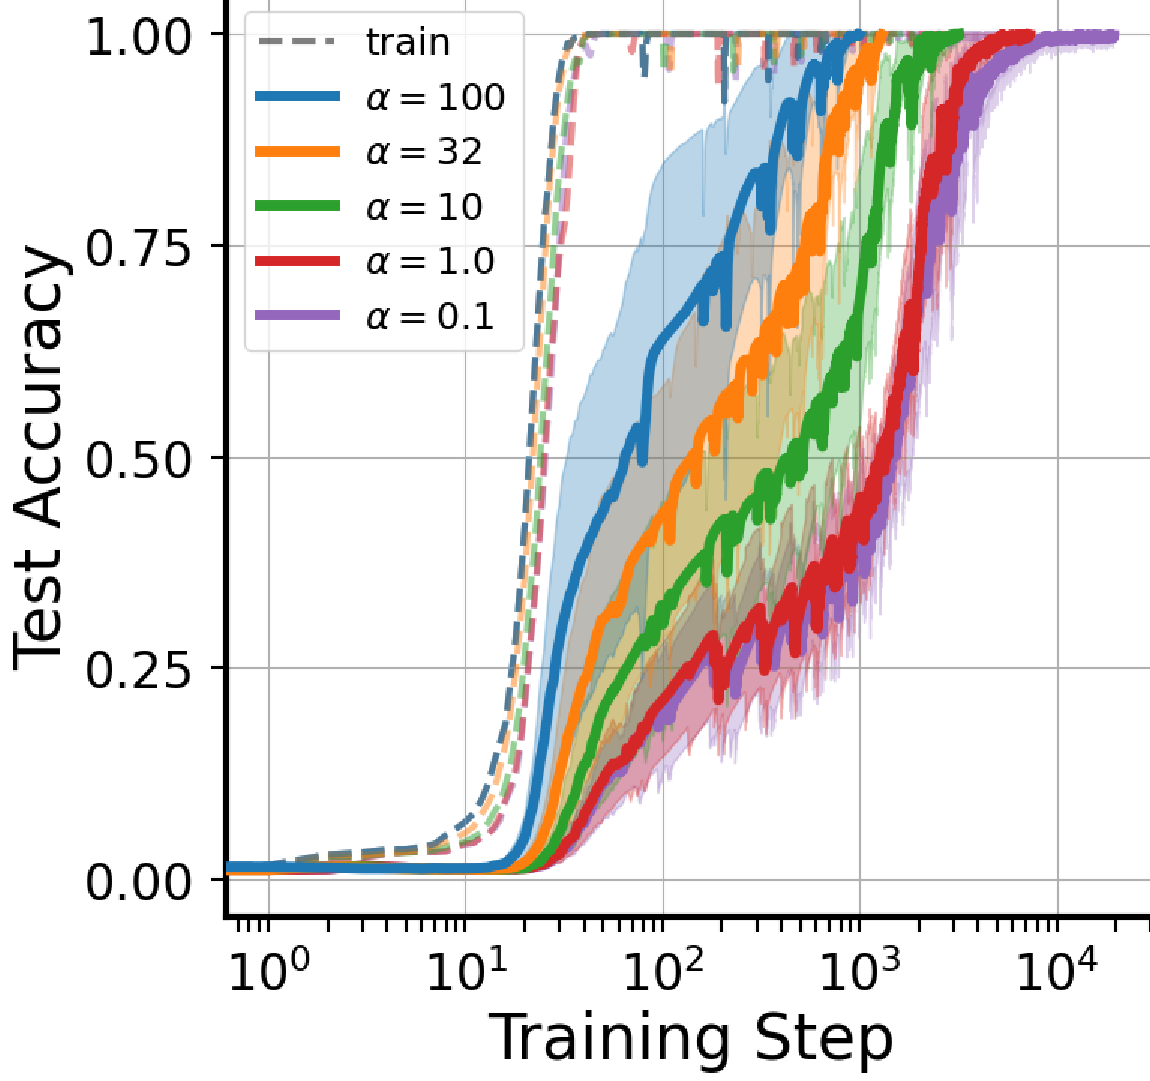
\includegraphics[width=\linewidth]{grokking_iclr_arxiv/figures/grokking.pdf}\vspace{-6mm}
\end{centering}
\caption{Our contributions demonstrated through results obtained in addition modulo 113 task. We show that the delay in generalization induced by NLM can be reversed using the proposed $\perp$\!AdamW ((\textbf{a}) and (\textbf{b})) and that the numerical errors that lead to overfitting instead of grokking can be avoided by using the proposed $\stablemax$ ((\textbf{b}) and (\textbf{c})). \vspace{-5mm}}
\label{fig:teaser}
%\vspace{-3mm}
\end{figure}

\begin{comment}
\begin{figure}[t]
\begin{subfigure}[t]{.32\textwidth}
    \includegraphics[width=\linewidth]{grokking_iclr/figures/teaser_baseline.pdf}
    \caption{AdamW}
\end{subfigure}
\hfill
\begin{subfigure}[t]{.32\textwidth}
    \includegraphics[width=\linewidth]{grokking_iclr/figures/teaser_softermax.pdf}
    \label{fig:input_representations}
    \caption{AdamW + stablemax}
\end{subfigure}%
\hfill
\begin{subfigure}[t]{.32\textwidth}
    \includegraphics[width=\linewidth]{grokking_iclr/figures/teaser_nlm.pdf}
    \label{fig:gradient_norms}
    \caption{$\perp$AdamW + stablemax}
\end{subfigure}
\caption{\vspace{-5mm}}
\vspace{-5mm}
\end{figure}
\end{comment}

% \vspace*{-2mm}
\section{Related work}
\label{sec:related}
% \vspace*{-2mm}
We review the most closely related work in this section.
For additional related work, see Appendix~\ref{appx:added_related}.
% \vspace*{-2mm}

\paragraph{Scaling laws.}
Early works on scaling artificial neural networks observe predictable power-law scaling in the training set size and number of model parameters~\cite{og_scaling,hestness2019beyond,rosenfeld_ConstructivePredictionGeneralization_2020}. 
\citet{alabdulmohsin2022revisiting} stress the importance of looking at the extrapolation regime of a scaling law.
\citet{yang2022tensor} prescribe architectural and hyperparameter changes when scaling model width to realize performant models; \citet{yang2023tensor} make analogous recommendations when scaling model depth.
\citet{Bi2024DeepSeekLS} propose hyperparameter aware scaling laws.
Unlike the aforementioned work, our investigation focuses on over-training and predicting downstream accuracy.

\citet{chinchilla} investigate how the number of model parameters $N$ and training tokens $D$ should be chosen to minimize loss $L$ given a compute budget $C$.
\citet{chinchilla} find that when scaling up $C$, both $N$ and $D$ should be scaled equally up to a multiplicative constant (i.e., $N \propto C^{\sim 0.5}$ and $D \propto C^{\sim 0.5}$) to realize compute-optimality.
Appendix C of the Chinchilla paper additionally suggests that these findings hold across three datasets.
However, \citet{chinchilla} do not verify their scaling laws for training beyond compute-optimality, or for downstream error prediction---both of which are central to our work. 

\citet{Sardana2023Beyond} propose modifications to the Chinchilla formulation to incorporate inference costs into the definition of compute-optimality and solve for various fixed inference budgets.
Their key finding, which is critical for our work, is that when taking into account a large enough inference budget, it is optimal to train smaller models for longer than the original Chinchilla recommendations.
Our work presupposes that over-training can be beneficial.
Instead of solving for inference-optimal schemes, we support empirically a predictive theory of scaling in the over-trained regime.
Additionally, we provide experiments across many validation and training sets.

For predicting downstream scaling beyond loss,~\citet{Isik2024ScalingLF} relate the number of pre-training tokens to downstream cross-entropy and machine translation BLEU score~\cite{papineni-etal-2002-bleu} after fine-tuning. 
In contrast, we take a holistic approach to evaluation by looking at top-1 error over many natural language tasks. 
\citet{schaeffer2023emergent} argue that emergent abilities~\cite{wei2022emergent} are a product of non-linear metrics and propose smoother alternatives.
As a warmup for why non-linear metrics may be hard to predict, \citet{schaeffer2023emergent} consider predicting an $\ell$ length sequence exactly: $\textsf{Err}(N, \ell) \approx 1 - \textsf{PP}(N)^{-\ell}$, where $N$ is the number of parameters in a model and $\textsf{PP}$ is its perplexity.
This is a special case of our Equations~\eqref{eq:errL} and~\eqref{eq:errPP}, where the number of training tokens does not appear, $\epsilon = 1, k = 1$, and $\gamma = \ell$.
In contrast, we treat $\epsilon, k, \gamma$ as free parameters for a scaling law fit, finding that average error over downstream tasks can make for a predictable metric.

\paragraph{Over-training in popular models.} There has been a rise in over-trained models~\cite{llama,llama2} and accompanying massive datasets~\cite{rpj,refinedweb,soldaini2024dolma,albalak2024survey}. For example, Chinchilla 70B~\cite{chinchilla} is trained with a token multiplier of 20, while LLaMA-2 7B~\cite{llama2} uses a token multiplier of 290.
In our investigation, we look at token multipliers from 5 to 640 to ensure coverage of popular models and relevance for future models that may be trained on even more tokens.
\section{Multimodal ArXiv}
This section presents a detailed construction process of our Multimodal ArXiv dataset, consisting of two sets: ArXivCap~(\S\ref{subsec:ArXivcap}) and ArXivQA~(\S\ref{subsec:arxiv_qa}).
% and then key statistics of the curated dataset.

% Figure~\ref{fig:chunk_example} illustrates a case sampled from our dataset.
% Step by Step?

% Use figure* for multi-column figure
\begin{figure*}[tp]
    \centering
    \includegraphics[width=0.95\linewidth]{figs/process.pdf}
    \caption{Overview of our dataset curation process. Starting from the ArXiv paper source files, we ensure the paper quality by selecting papers according to publication records. Figure and caption pairs are extracted and then cleaned according to manually designed rules. ArXivQA is generated by prompting GPT-4V with a curated template.}
    \label{fig:dataset-curation-process}
\end{figure*}


\subsection{ArXivCap}
\label{subsec:ArXivcap}

% \subsubsection{Construction Process of ArXivCap}
\paragraph{Construction Process} We outline the creation process of ArXivCap below and Figure~\ref{fig:dataset-curation-process} gives an overview.

\noindent\emph{Paper Filtering with Publication Type:}
\DatasetName is extracted from ArXiv~\cite{clement2019use}, which is under CC-0 licence for modification and distribution. 
% Therefore, we have the permission to create and distribute \DatasetName. 
% The files in the ArXiv dataset are in tar format, which includes LaTeX files and their corresponding image files. 
The raw files of papers posted on ArXiv tar files before June 2023 are downloaded. 
To ensure the quality of our dataset, we employ a rigorous selection process to filter potentially low-quality papers that might influence the figure-caption pair quality. 
Firstly, we retrieve meta-information for papers from Semantic Scholar~\cite{kinney2023semantic}, which contains the publication record for each paper. 
Papers with publication types \texttt{JournalArticle},  \texttt{Conference}, or \texttt{Review} are kept as we assume the peer-review process could ensure the overall figure-caption quality is satisfactory.
We further exclude papers with titles exceeding 100 words or abstracts longer than 300 words, in alignment with common submission requirements.
% We further filter out papers with titles longer than 100 words, or with an abstract longer than 300 words, according to common submission requirements.
% for examples. 
% There are 2,285,111 papers and 13,945,502 images in total till this step.


% % Use figure* for multi-column figure
\begin{figure}[!t]
    \centering
  \begin{subfigure}{0.45\textwidth}
    \centering
    \includegraphics[width=\textwidth]{figs/examples/1-1.png}
    \caption{Single Figure-Caption}
    \label{fig:subfig1}
  \end{subfigure}
  \hfill
  \begin{subfigure}{0.45\textwidth}
    \centering
    \includegraphics[width=\textwidth]{figs/examples/1-2.png}
    \caption{Multiple Figure-Caption}
    \label{fig:subfig2}
  \end{subfigure}
  \caption{Chunk Example. \lilei{add case of arxiv qa}}
  \label{fig:chunk_example}
\end{figure}

% \paragraph{Unify Image Format} 
% We utilize ImageMagisk~\cite{imagemagick} to convert images of various formats, including .ps, .epsi, .PS, .pdf, .PDF, .EPS, .eps, etc., into the JPEG format, while preserving the original jpg/jpeg and png images. ImageMagisk is a robust tool for image editing and transformation. Additionally, we standardize the output format to jpg/jpeg in RGB mode and remove the white border around images.

% according to our prior.
% This ensures that we include papers published in reputable journals, conference proceedings, or recognized review articles.
% We further keep papers satisfying the following requirements:
\noindent\emph{Figure-Caption Pair Extraction:}
Images and captions are extracted from the original LaTeX files by matching the syntax. 
We further use a robust tool ImageMagisk~\cite{imagemagick} to convert images into JPEG format for easy processing.
The extracted images and captions are stored in a designed chunk structure,
which consists of either a single figure-caption pair or multiple figures with their respective sub-captions and a main caption for the overall description.
This format is more consistent with the layout of academic papers, and
Figure~\ref{fig:chunk_example} illustrates the chunk structure.

% \begin{enumerate}% [leftmargin=2em]
%     \item The number of words in the abstract is in  $[10, 300]$.
%     \item The number of words in the title is in $[1, 100]$.
% \end{enumerate}

\begin{figure}[t!]
    \centering
    \includegraphics[width=0.9\linewidth]{figs/chunk-v2.pdf}
    \caption{Illustration of two types of figure-caption pairs. (Left) Single-Figure pair. (Right) Multiple-Figure caption pair has multiple sub-figures with corresponding sub-captions and an overall main caption. }
    \label{fig:chunk_example}
\end{figure}
% \paragraph{Filter Images}
% After resizing images using Lanczos resampling, we ensure that the maximum dimension of each image does not exceed 2016 pixels. Following a manual inspection of the images, we apply the following filters to refine the selection process further, retaining only the images that meet the specified requirements:

% \begin{enumerate}
%     \item The ratio between the width and height of the image is less than 100.
%     \item The width or height of the image is larger than 224 pixels.
%     \item The number of pixels in the image is less than 89,478,485.
% \end{enumerate}


\noindent\emph{Caption Cleaning and Image Filtering:}
After a manual inspection of the initially collected dataset, we design several transformations to clean the captions and filter the images.

\noindent\emph{Caption Cleaning}: (i) Chunks with captions shorter than 5 words are removed; (ii) For captions with LaTeX expressions such as math formulas and references, we apply the \texttt{pylatexenc}\footnote{https://github.com/phfaist/pylatexenc} to transform the LaTeX to text with math formulas retained, citations to a special symbol \texttt{<cit.>}, references to \texttt{<ref>}. An illustration of caption cleaning can be found in Appendix~\ref{apx:caption_clean}.
%\textgreater"


\noindent\emph{Image Filtering}: We remove images that are deemed to be problematic according to the following rules:
(i) Images with an aspect ratio larger than 100; (ii) Images with the shortest edge shorter than 224 pixels; and (iii) Images with pixel numbers larger than the decompression bombs threshold.
% The ratio between the width and height of the image is less than 100.
%     \item The width or height of the image is larger than 224 pixels.
%     \item The number of pixels in the image is less than 89,478,485.
% Replace incorrect newline characters with empty spaces.
    % \item Replace consecutive empty spaces with a single space.
    % Remove chunks that have captions with fewer than 5 words or no words at all.
   % Utilize pylatexenc to convert LaTeX to text, ensuring that math formulas are retained. Additionally, normalize citations and tables to "\textless ref \textgreater" and "\textless cit. \textgreater" format. (\cref{tab:pylatexenc_clean})
% \end{enumerate}

After these processes, 100 pairs are sampled to perform an additional manual inspection, where we found all of these pairs contained clear images and correct caption descriptions. We provide visualized figure-caption pairs in Appendix~\ref{apx:case_illustrations}.
\paragraph{Statistics of ArXivCap}
% In this section, we present a general analysis of \DatasetName. Detailed analysis can be found in the Appendix. 

% \begin{table*}[ht!]
    
%     \centering
    
%     \small 
%     \begin{tabular}{@{}lcccccc@{}}
%          \toprule
%         Field & Number & Total & Average & Minimum & Maximum & Quartile \\
%          \midrule
         
%         Title & 572,734 & 5,960,728 & 10.41 & 1 & 100 & (8, 10, 12) \\
                 
%         Abstract & 572,734 & 95,987,566 & 167.6 & 10 & 300 & (126, 165, 207) \\
        
%         Chunk Caption & 3,963,576 & 193,482,743 & 48.82 & 1 & 2,248 & (16, 36, 67) \\
        
%         Main Caption & 3,958,840 & 188,590,156 & 47.64 & 1 & 2,248 & (15, 35, 65) \\

%         Subcaption & 1,025,704 & 4,892,587 & 4.77 & 1 & 307 & (2, 3, 5) \\  

%         Images & 6,481,222 & N / A & N / A & N / A & N / A & N / A \\
%          \bottomrule
%     \end{tabular}
%     \caption{Word count statistics for title, abstract, captions and Image number. A word is defined as any sequence of characters matching the regular expression pattern r"\textbackslash w+". \cref{fig:chunk_example} shows the example of subcaption and main caption. The term "Chunk caption" encompasses all captions within it, including both the subcaption and the main caption contained within it.}
%     \label{tab:detail_statistic_title_abstract_image_caption}
% \end{table*}

\begin{table}[t!]
    \centering
    \resizebox{\linewidth}{!}{
    \begin{tabular}{@{}lccc@{}}
         \toprule
        Field & Number &  Average Len.  & Quartile of Len. \\
         \midrule
         
        Title & 572K &  10.4   & (8, 10, 12) \\ 
        Abstract & 572K &  167.6  & (126, 165, 207) \\
        \midrule 
        Main Caption & 3.9M  &  47.6 & (15, 35, 65) \\
        Subcaption & 1.0M  & 4.8 &  (2, 3, 5) \\  
        Chunk Caption & 3.9M &  48.8  & (16, 36, 67) \\
        \midrule 
        Images & 6.4M  & N / A  & N / A \\
         \bottomrule
    \end{tabular}}
    \caption{Word count statistics for title, abstract, captions, and Image number. 
    Chunk caption refers to the combination of subcaptions and the main caption for a multiple-figure case.}
    \label{tab:detail_statistic_title_abstract_image_caption}
\end{table}

\begin{table*}[ht!]
    \centering
\resizebox{\textwidth}{!}{
    \begin{tabular}{@{}lccccc@{}}
         \toprule
        Dataset & Image Number & Paper Number & Image Category & Domain & Real Data \\
         \midrule
                 FigCAP~\citep{chen2020figcap} & 219K & N / A & Bar, Line and Pie Charts & N / A & \xmark \\
        
         SciCap~\citep{Yang2023SciCap+} & 2.1M & 295K & Open-Category & Computer Science and Machine Learning & \cmark \\

         M-Paper~\citep{hu2023mplugpaperowl} & 350K & 48K & Open-Category & Mainly "Deep Learning" & \cmark \\   
        
         ArXivCap (Ours) & 6.4M & 572K & Open-Category & Open-Domain & \cmark \\
 
        \midrule 
FigureQA~\citep{kahou2017figureqa}  & 140K & N / A & Bar, Line and Pie Charts & N / A & \xmark \\
                 
        DVQA~\citep{kafle2018dvqa} & 300K & N / A & Bar Charts & N / A& \xmark \\
         ArXivQA (Ours) &  32K & 16.6K & Open-Category & Open-Domain & \cmark \\
         \bottomrule
    \end{tabular}}
    \caption{Comparison with previous scientific figure datasets. Our ArXivCap is the largest captioning dataset and our ArXivQA is the only QA dataset that covers a wide range of domains from real papers. }
    \label{tab:dataset_comparison_1}
\end{table*}

% \crossmark & \cmark 

Table~\ref{tab:detail_statistic_title_abstract_image_caption} lists the dataset statistics. 
ArXivCap consists of 572K papers, containing 6.4M high-quality images in total with 193M words. 
A word cloud illustration of captions can be found in the Appendix~\ref{apx:caption_word_cloud}.
Figure~\ref{fig:domain-distribution} demonstrates the paper domain distribution extracted from ArXiv, where we find that our ArXivCap covers 32 domains, such as computer science, mathematics, physics, and economics.
As shown in Table~\ref{tab:dataset_comparison_1}, compared with previous scientific figure datasets, our ArXivCap is the largest figure-caption dataset collected from real papers and covers a wide range of scientific domains, serving as a valuable resource for improving and benchmarking LVLMs.

%, and our ArXivQA is the only open-domain QA datasets with diverse figure types.

% , providing a comprehensive general knowledge for LVLMs.

% It is the largest image-caption dataset for academic figures, encompassing a diverse array of domains and image categories. \cref{tab:dataset_comparison_1} presents comparison between \DatasetName and other datasets.
 % We get the domain category for each paper from \cite{ArXiv.org_submitters_2023}. 



% \begin{table}[tbh!]
    \centering
    \begin{tabular}{l|c}
    \toprule
       Field  & Total Number \\
       \midrule
       Title \& Abstract & 572,734 \\ 
       Image & 6,481,222 \\ 
       Caption & 3,961,133 \\ 
       \bottomrule
    \end{tabular}
    \caption{Data Statistics of the curated dataset.}
    \label{tab:data_statistics}
\end{table}

\begin{table}[tbh!]
    \centering
    \begin{tabular}{l|cc}
    \toprule
       Field  & Total Number & Word Number \\
       \midrule
       Block Caption & 3,963,576 & 193,482,743 \\ 
       Main Caption in Block & 3,958,840 & 188,590,156 \\ 
       Subcaption in Block & 1,025,704 & 4,892,587 \\ 
       \bottomrule
    \end{tabular}
    \caption{Caption Statistics of the curated dataset.}
    \label{tab:caption_statistics}
\end{table}


% \begin{table}[tbh!]
%     \centering
%     \begin{tabular}{l|cc}
%     \toprule
%        Field  & Statistic \\
%        \midrule
%        Image Number & 6,481,222 \\ 
%        Total Size & 892GB \\ 
%        \bottomrule
%     \end{tabular}
%     \caption{Image Statistics of the curated dataset.}
%     \label{tab:image_statistics}
% \end{table}


\input{figs/domain-distribution}

\subsection{ArXivQA}
\label{subsec:arxiv_qa}
As our ArXivCap contains diverse images from scientific domains, we assume that learning to answer questions about these figures could boost scientific reasoning ability. Following the successful practice of LLaVA~\citep{liu2023llava}, we adopt GPT-4V to generate instruction-tuning datasets for generating the QA pairs based on the figures extracted from scientific papers.
Specifically, we design a prompting template to query GPT-4V for generating QA pairs based on 35K images randomly sampled from our ArXivCap.
Table~\ref{tab:prompt_for_ArXivqa} in Appendix~\ref{apx:prompt_template} provides the template we used for the prompt.
The generated pairs are parsed according to the format requirement and we discard the samples without options and rationales.
There are 100K QA pairs after filtering the invalid samples. 
The dataset comprises questions with an average word count of 16.98 for the question text.
% and options for the question with an average word count of 31.86. 
On average, there are 4.20 options per question and the average length of the text for a single option is 7.59 words.
Appendix~\ref{apx:case_illustrations} provides samples from the ArXivQA dataset.

As a preliminary study, we sample 1,000 samples from ArXivQA and prompt open-sourced LVLMs to predict answers given the questions and options. 
A simple prompt is designed to employ GPT-4 for extracting the answer label from the model generations.
For human performance, we ask four authors to perform predictions on a 100-sample subset (where 17 samples are from the CS domain). Each of them is asked to answer 50 samples and the accuracy scores are obtained by averaging two annotators.
As shown in Table~\ref{tab:arxiv_qa_acc}, most models struggle to perform satisfactorily on the ArXivQA dataset, falling far behind human performance. This verifies our premise that current open-sourced LVLMs fail to understand scientific figures. We also notice that simply increasing the model scale from 7B (LLaVa-1.5-7B) to 13B (LLaVa-1.5-13B) does not yield a significant boost, which indicates that the ability for multimodal mathematical reasoning cannot be simply acquired from the LLM-side only. 




\begin{table}[t!]
    \centering
    \small 
    \begin{tabular}{l|c}
        \toprule
        Model & Accuracy \\
        \midrule
        InstructBLIP-Vicuna7B & 7.0\% \\
        LLaVA-1.5-7B & 44.2\% \\
        LLaVA-1.5-13B & 46.8\% \\
        OpenFlamingo-9B & 9.9\% \\
        IDEFICS-Instruct-9B & 34.5\% \\
        Qwen-VL-Chat & 46.6\% \\
        \midrule 
        \textcolor{gray}{Human (100-sample Subset)} & \textcolor{gray}{80.0\%} \\
        \textcolor{gray}{Human (CS subset)} & \textcolor{gray}{88.2\%} \\
        \bottomrule
    \end{tabular}
    \caption{Evaluation results on the sampled 1,000 ArXivQA samples. }
    \label{tab:arxiv_qa_acc}
\end{table}
% Domain and Option Number, Option length, verb visualization?




%---------------------------------
\vspace{-0.3em}
\section{Experimental Results}
\label{sec:result}
%---------------------------------

%---------------------------------
\subsection{Experimental settings}
\label{subsec:experiment_setting}
%---------------------------------

\paragraph{Implementation Details.} 
We adopt the VideoCrafter~\cite{chen2023videocrafter} as our base T2V model, which shares the same spatial weights with Stable Diffusion 2.1. We first train the style modulation on image dataset, i.e. WikiArt~\cite{phillips2011wiki} and Laion-Aesthetics-6.5+~\cite{schuhmann2022laion} for 40k steps with a batch size of 32 per GPU.  In the second stage, we froze the style modulation part and only train temporal blocks of VideoCrafter, we jointly train image datasets and video datasets(subset of WebVid-10M~\cite{bain2021frozen}) for 20k steps with a batch size of 1 on video data and 16 on image data, sampling image batches with a ratio of 20\%. The training process is performed on 8 A100 GPUs and can be completed within 3 days. Furthermore, to ensure a fair comparison with some SDXL-based models~\cite{ye2023ipadapter, hertz2023style} on stylized image generation, we also trained the first stage of StyleCrafter on SDXL~\cite{podell2023sdxl}. 
%The overall training process takes about 5 days on 8$\times$V100.

% We train the style adapter on xx for xx epoches, with xx frozen and only train xxxx. In the second stage, xxx. We use xx optimizer and learning rate of xxxx. Also, training dataset.  \TODO{complete this part}

\paragraph{Testing Datasets.}
\label{sec:test_dataset}
To evaluate the effectiveness and generalizability of our method, we construct testsets comprising content prompts and style references. For content prompts, we use GPT-4~\cite{openai2023gpt4v} to generate recognizable textual descriptions from four meta-categories~(human, animal, object, and landscape). We manually filter out low-quality prompts, retaining 20 image prompts and 12 video prompts. For style references, we collect 20 stylized images and 8 sets of style images with multi-reference~(each contains 5 to 7 images in similar styles) from the Internet. In total, the test set contains 400 pairs for stylized image generation, and 300 pairs for stylized video generation (240 single-reference pairs and 60 multi-reference pairs). Details are available in the supplementary materials.

% 1. Content Prompt(generated from GPT4)
% 2. Style Image(selected from internet)
% 3. Content Image(generated from SD, for some style transfer method)
% 4. Style Prompt(generated from GPT4-v, for sd and video-crafter)

\paragraph{Evaluation Metrics.}
\label{sec:eval_metrics}
Following previous practice~\cite{zhang2023inversion, sohn2023styledrop, wang2023styleadapter}, we employ CLIP-based~\cite{radford2021learning} scores and DINO-based~\cite{caron2021emerging} scores to measure the text alignment and style conformity. Following EvalCrafter~\cite{liu2023evalcrafter}, we measure the temporal consistency of video generation by (i) calculating clip scores between contiguous frames and (ii) calculating the warping error on every two frames with estimated optical flow. 
Note that these metrics are not perfect. For example, one can easily achieve a close-to-1 style score by entirely replicating the style reference. Similarly, stylized results may yield inferior text scores compared to realistic results, even though both accurately represent the content descriptions. We recommend a comprehensive consideration of both CLIP-based text scores and style scores, rather than relying solely on a single metric.

\paragraph{User Preference Study.}
In addition to quantitative analysis, we conducted a user study to make comparisons among our method, VideoCrafter, Gen-2, and AnimateDiff in the context of single-reference and multi-reference stylized video generation. Users are instructed to select their preferred option based on style conformity, temporal quality, and all options fulfill text alignment for each comparison pair. We randomly chose 15 single-reference pairs and 10 multi-reference pairs, collecting 1125 votes from 15 users. 
Further details can be found in the supplementary materials.

%
\begin{table*}[!t]
\centering
%\setlength{\tabcolsep}{3.0pt}
% \renewcommand\arraystretch{1.5}
\caption{Quantitative comparison on single-reference style-guided T2I generation. We conduct evaluation on a test set of 400 pairs. \textbf{Bold}: Best. }
\label{tab:img_quan_clip}
\vspace{-1em}
\resizebox{0.93\linewidth}{!}{
  \begin{tabular}{ccccccccc} % {@{}lc@{}}
    \toprule
     \multirow{2}{*}{Method} & \multicolumn{4}{c}{\textbf{Stable Diffusion 2.1 based}} & \multicolumn{4}{c}{\textbf{SDXL based}} \\
    \cmidrule(lr){2-5}\cmidrule(lr){6-9}
     & Dreambooth & InST & SD* & Ours & IP-Adapter-Plus & Style-Aligned & SDXL* & Ours(SDXL)  \\
    \midrule
    \texttt{CLIP-Text} $\uparrow$ & \textbf{0.3047}  & 0.3004 & 0.2766 & 0.3028 & 0.2768 & 0.2254 & 0.2835 & \textbf{0.2918} \\
    \texttt{CLIP-Style} $\uparrow$ & 0.3459 & 0.3708 & 0.4183 & \textbf{0.4836} & 0.5182 & 0.5515 & 0.4348 & \textbf{0.5615} \\
    \texttt{DINO-Style} $\uparrow$ & 0.2278 & 0.2587 & 0.2890 & \textbf{0.3652} & 0.4367 & 0.4395 & 0.2912 & \textbf{0.4514} \\
    \bottomrule
  \end{tabular}
}
\end{table*}



%---------------------------------
\subsection{Style-Guided Text-to-Image Generation}
\label{subsec:image_eval}
%---------------------------------

As mentioned in Sec.~\ref{subsec:style_modulation} and Sec.~\ref{subsec:experiment_setting}, our proposed method also supports to generate stylized images~(using model before temporal finetuning). We are interested to evaluate our method against state-of-the-art style-guided T2I synthesis methods, which are better-established than video counterparts. The competitors include optimization-based methods like DreamBooth~\cite{dreambooth}, inversion-based methods such as InST~\cite{zhang2023inversion} and Style-Aligned~\cite{hertz2023style}, and adapter-based methods like IP-Adapter-Plus~\cite{ye2023ipadapter}. Besides, we consider two unique competitors: SD*~\cite{ldm} and SDXL*~\cite{sdxl}~(text-to-image models equipped with GPT-4V~\cite{openai2023gpt4v}, where GPT-4V generates textual descriptions about the reference's style and merges them with content prompts as input for models). This comparison aims to validate the advantages of employing image conditions to enhance stylized generation instead of relying solely on text conditions.
Implementation details of competitors are available in supplementary materials.
% For each style, DreamBooth and CustomDiffusion are optimized with the provided single reference image to learn the customized concept of style.
%This setting may degrade their performance (because they usually requires 5~20 images to learn a concept) but it is fair comparison since all the methods are only provided with a single style image.

The quantitative comparison is tabulated in Table~\ref{tab:img_quan_clip}. 
% Although our method achieved the best performance on both metrics, we would like to emphasise that clip-based metrics are imperfect.As discussed in Sec.~\ref{sec:eval_metrics}, the CLIP-Text is measured by the similarity between content text embedding and stylized image embedding, the stylistic appearance actually hinders the metric in some extent, which makes those methods with weak stylistic effects (i.e. close to photorealism) achieve superior scores. 
Results reveal that Dreambooth~\cite{dreambooth} and InST~\cite{zhang2023inversion} struggle to accurately capture the style from various style references and exhibit low style conformity. SD*~\cite{ldm} and SDXL~\cite{sdxl} demonstrate good stylistic ability but still fail to reproduce the style of the reference image, possibly because of the text’s inherent clumsiness in expressing specific styles despite utilizing the powerful GPT4V for visual style understanding. IP-Adapter~\cite{ye2023ipadapter} and style-aligned~\cite{hertz2023style} generate aesthetically pleasing images, while their style-content decoupled learning is not perfect and exhibits limited control over content.
In contrast, our method efficiently generates high-quality stylized images that align with the content of the texts and resemble the style of the reference image. Our method demonstrates stable stylized generation capabilities when dealing with various types of prompts.


%---------------------------------
\subsection{Style-Guided Text-to-Video Generation}
\label{subsec:video_eval}
%---------------------------------

\begin{figure*}[t!]
    \centering
    \includegraphics[width=0.87\linewidth]{figures/comp_image.pdf}
    \vspace{-1em}
    % \vspace{-2em}
    \caption{Visual comparison on style-guided T2I generation. \textcolor[RGB]{46, 117, 182}{Blue}: methods based on SD 2.1. \textcolor[RGB]{84, 130, 53}{Green}: based on SDXL. Prompt: A rabbit nibbling on a carrot.} 
    \label{fig:result_img}
    \vspace{-1em}
\end{figure*}
%
\begin{figure*}[!h]
    \centering
    \includegraphics[width=0.9\linewidth]{figures/comp_video.pdf}\vspace{-1.5em}
    \caption{Visual comparison of single-reference guided T2V generation. Vid.Comp.: VideoComposer, Vid.Craf.: VideoCrafter
    %Our approach accurately captures the style of the reference image and generates videos that satisfy both text alignment and style conformity.
    } 
    \label{fig:result_video}
    \vspace{-1em}
\end{figure*}
%
\begin{figure*}[!h]
    \centering
    \includegraphics[width=0.87\linewidth]{figures/comp_video2.pdf}
    \vspace{-1em}
    \caption{Qualitative comparison of multi-reference style-guided T2V generation. S-R: Single-Reference, M-R: Multi-Reference
    %AnimateDiff tends to generate close-to-reamlism results despite the style references are typical artistic styles. In contrast, our approach performs better in text alignment, style conformity and temporal consistency.
    } 
    \vspace{-1em}
    \label{fig:result_multi_ref}
\end{figure*}



\begin{table}[!t]
\centering
\caption{Quantitative comparison of style-guided T2V generation. Top 3 rows: single-reference based gudiance. Bottom 3 rows: multi-reference based guidance. S-R: Single-Refernce, M-R: Multi-Reference, W.E.: Warping Errors.}
\label{tab:video_quan_clip}
\vspace{-1em}
\resizebox{\linewidth}{!}{
% \scriptsize
% \renewcommand\arraystretch{1.2}
\begin{tabular}{c c c cc} % {@{}lc@{}}
    % \toprule
    \toprule
    \multirow{2}{*}{Methods} & \multirow{2}{*}{CLIP-Text $\uparrow$} & \multirow{2}{*}{CLIP-Style $\uparrow$} & \multicolumn{2}{c}{Temporal Consistency} \\
    \cmidrule(lr){4-5}
      & & &
     ~CLIP-Temp $\uparrow$~ & \makecell{W.E.($\times10^{-3}$) $\downarrow$}\\
    \midrule
    VideoComposer & 0.0468 & \textbf{0.7306} & 0.9853 & \textbf{9.903} \\
    VideoCrafter* & 0.2209 & 0.3124 & 0.9757 & 61.41 \\
    Ours & \textbf{0.2726} & 0.4531 & \textbf{0.9892} & 18.73 \\
    \midrule
    ~AnimateDiff & \textbf{0.2867} & 0.3528 & 0.8903 & 37.17 \\
    Ours(S-R) & 0.2661 & 0.4803 & 0.9851 & 14.13 \\
    Ours(M-R) & 0.2634 & \textbf{0.4887} &\textbf{0.9852} & \textbf{9.396} \\
    \bottomrule
  \end{tabular}
}
\end{table}

\begin{table}[!t]
\centering

\caption{User study statistics of the selection rate for text alignment(\texttt{Text}), and preference rate for style conformity(\texttt{Style}) and temporal quality(\texttt{Temporal}). Top 3 rows: single-reference based guidance. Bottom 2 rows: multi-reference based guidance.}
\label{tab:video_quan_multi_ref}
\vspace{-1em}

\small
\begin{tabular}{c c c c} % {@{}lc@{}}
    % \toprule
    \toprule
    Methods & \texttt{Text} $\uparrow$ & \texttt{Style} $\uparrow$ & \texttt{Temporal} $\uparrow$ \\
    \midrule
    VideoCrafter* & 0.391 & 8.0\% & 4.4\%  \\
    Gen-2* & 0.747 & 23.1\% & 51.1\% \\
    Ours & 0.844 & 68.9\% & 44.4\% \\
    \midrule
    ~AnimateDiff~ & 0.647 & 10.0\% & 19.3\% \\
    Ours(M-R) & 0.907 & 90.0\% & 80.7\% \\
    \bottomrule
\end{tabular}
\end{table}

Existing approaches for style-guided video generation can be divided into two categories: one is the single-reference based methods that are usually tuning-free, e.g. VideoComposer~\cite{wang2024videocomposer}; the other is the multi-reference based methods that generally requires multiple references for fine-tuning, e.g. AnimateDiff~\cite{guo2023animatediff}. We make comparisons with these methods, respectively. 
% Apart from the quality metrics, we further conduct user study to evaluate the stylized video results, including text alignment, style conformity and temporal quality.


\vspace{-0.5em}
\paragraph{Single-Reference based Guidance.}VideoComposer~\cite{wang2024videocomposer} is a controllable video generation model that allows multiple conditional inputs including style reference image. It is a natural competitor of our method. 
Besides, we construct two additional comparative methods, i.e. VideoCrafter* and Gen2*, which extend VideoCrafter~\cite{chen2023videocrafter} and Gen2~\cite{Gen-2}, the state-of-the-art T2V models in open-source and close-source channels respectively, to make use of style reference images by utilizing GPT-4V~\cite{openai2023gpt4v} to generate style prompts from them.
% The evaluation is conducted on 240 text-style pairs, as introduced in Sec.~\ref{sec:test_dataset}. 
The quantitative comparison is tabulated in Table~\ref{tab:video_quan_clip}. Several typical visual examples are illustrated in Figure~\ref{fig:result_video}.

We can observe that: 
(i) VideoComposer tends to copy content from style references and struggles to generate text-aligned content, which is possibly because of the invalid decoupling learning. Consequently, its results exhibit abnormally high style conformity and very low text alignment. In addition, VideoComposer often generates static videos, thus having the lowest warping errors, but this does not mean that their results perform best in temporal quality. 
(ii) VideoCrafter* exhibits limited stylized generation capabilities, producing videos with diminished style and disjointed movements. Gen-2* demonstrates superior stylized generation capabilities. However, Gen-2 is still limited by the inadequate representation of style in textual descriptions, and is more prone to sudden changes in color and luminance. (iii) In comparison, our method captures styles more effectively and reproduces them in the generated results.

\begin{figure}[!t]
    \centering
    \includegraphics[width=\linewidth]{figures/ablation_img_1.pdf}
    \vspace{-3em}
    \caption{Effects of dual cross-attention and data augmentation.} 
    \label{fig:ablation_img_1_2}
    \vspace{-1em}
\end{figure}


\vspace{-0.5em}
\paragraph{Multi-Reference based Guidance.}
AnimateDiff~\cite{guo2023animatediff} denotes a paradigm to turn personalized SD (i.e., SD fine-tuned on specific-domain images via LoRA~\cite{hu2022lora} or Dreambooth~\cite{dreambooth}) for video generation, namely combined with pre-trained temporal blocks of T2V models. It can generate very impressive results if the personalized SD is carefully prepared, however, we find it struggle to achieve as satisfactory results if only a handful of style reference images are available for training.
We conduct an evaluation on 60 text-style pairs with multi-references, as presented in Sec.~\ref{sec:test_dataset}. We train Dreambooth~\cite{dreambooth} models for each style and incorporate them into AnimateDiff based on their released codebase. Thanks to the flexibility of Q-Former, our method also supports multiple reference images in a tuning-free fashion, i.e. computing the image embeddings of each reference image and concatenating all embeddings as input to the Q-Former.
Results are compared in Table~\ref{tab:video_quan_multi_ref} and Figure~\ref{fig:result_multi_ref} respectively.

According to the results, AnimateDiff struggles to achieve high-fidelity stylistic appearance while tends to generate close-to-realism results despite the style references are typical artistic styles. In addition, it is vulnerable to temporal artifacts. As the trained personalized-SD can generate decent stylistic images (provided in the supplementary materials), we conjecture that the performance degradation is caused by the incompatibility from the pre-trained temporal blocks and independently trained personalized-SD models, which not only interrupts temporal consistency but also weakens the stylistic effect.
In contrast, our method can generate temporal consistent videos with high style conformity to the reference images and accurate content alignment with the text prompts. Furthermore, using multiple references can further promote the performance, which offers additional advantages in practical applications.


%---------------------------------
\subsection{Ablation Study}
\label{subsec:ablation}
%---------------------------------

\begin{figure}[!t]
    \centering
    \includegraphics[width=\linewidth]{figures/ablation_no_scale.pdf
    }
    \vspace{-2em}
    \caption{Effect of adaptive content-style fusion. It shows superiority in generalization to extreme cases, e.g. long text description. Two text prompts are used: (i) A little girl; (ii) \textit{A little girl \textcolor[RGB]{255, 64, 255}{reading a book} in the park, with \textcolor[RGB]{244, 177, 131}{a telescope} nearby pointed at the sky}.}
    \label{fig:ablation_no_fusion}
    \vspace{-0.7em}
\end{figure}

% We make ablation studies on some important designs of our method, including data augmentation, module architectures, and training strategies, to validate their effectiveness.

\paragraph{Data Augmentation.}
We first study the effectiveness of content-style decoupled data augmentation. As depicted in Table~\ref{tab:ablation_img}, training with the original image-caption pairs restricts the model's ability to extract style representations, leading to lower style conformity. For example, as shown in Figure~\ref{fig:ablation_img_1_2}, method without data augmentation fails to capture the "3D render" style from the reference.


\paragraph{Dual Cross-Attention.} 
As discussed in Sec.~\ref{subsec:style_modulation},  we make a comparison between \textit{attach-to-text} and \textbf{dual cross-attention} to study their effects. Results are presented in Table ~\ref{tab:ablation_img} and Figure~\ref{fig:ablation_img_1_2}, revealing that \textit{attach-to-text} tends to directly fuse the content from the reference image and the text prompts rather than combining the text-based content and image-based style. This indicates the effectiveness of \textbf{dual cross-attention} in facilitating content-style decoupling.


\paragraph{Adaptive Style-Content Fusion.}
As previously discussed in Figure~\ref{fig:scale_factor_viz}, our proposed adaptive style-content fusion module demonstrates effectiveness in adaptively processing various conditional contexts. It benefits the generalization ability of model to deal with diverse combinations of content prompt and style image. Figure~\ref{fig:ablation_no_fusion} reveals that although the baseline can handle easy prompt inputs like "A little girl", it struggles to accurately generate all objects described in longer prompts. In contrast, the adaptive fusion module can achieve decent text alignment for long text descriptions thanks to its flexibility to adaptive balance between content and style.

\paragraph{Two-Stage Training Scheme.}
Our proposed training scheme consists of two stages, i.e., style adapter training and temporal adaption. To show its necessity, we build two baselines: (i) \textit{w/o Temporal Adaption}: that we train a style adapter on image data and apply it directly to stylized video generation without finetuning; (ii) \textit{joint training}: that we conduct style adapter training and temporal blocks finetuning on image-video dataset simultaneously.
As depicted in Table~\ref{tab:ablation_video}, baseline (i) exhibits inferior temporal consistency when applied directly to video, and undermines the content alignment and style conformity. As for baseline (ii), the learning of style embedding extraction seems to be interfered by the joint finetuning of temporal blocks, which impedes it to generate desirable stylized videos.


\begin{table}[!t]
\centering

\caption{Ablation studies on style modulation designs. The performance is evaluated based on the style-guided T2I generation.}
\label{tab:ablation_img}
\vspace{-1em}
    
\small
% \renewcommand\arraystretch{1.2}
  \begin{tabular}{ccc} % {@{}lc@{}}
    % \toprule
    \hline
    Methods & \texttt{CLIP-Text} $\uparrow$ & \texttt{CLIP-Style} $\uparrow$ \\
    \hline
    Ours & 0.3028 & 0.4836 \\
    ~w/o Data Augmentation & 0.3173 & 0.4005 \\
    w/o Dual Cross Attention & 0.0983 & 0.7332 \\
    w/o Adaptive Fusion & 0.2807 & 0.4925 \\
    \hline
  \end{tabular}
\vspace{-1em}
\end{table}


\begin{table}[!t]
\centering
\vspace{1em}

\caption{Ablation study on our two-stage training scheme.}
\vspace{-1em}
\label{tab:ablation_video}
% \renewcommand\arraystretch{1.5}
\resizebox{\linewidth}{!}{

\begin{tabular}{c c c cc} % {@{}lc@{}}
    % \toprule
    \toprule
    \multirow{2}{*}{Methods} & \multirow{2}{*}{CLIP-Text $\uparrow$} & \multirow{2}{*}{CLIP-Style $\uparrow$} & \multicolumn{2}{c}{Temporal Consistency} \\
    \cmidrule(lr){4-5}
      & & &
     ~CLIP-Temp $\uparrow$~ & \makecell{W.E.($\times10^{-3}$) $\downarrow$}\\
    \midrule
    w/o Temporal Adaption  & 0.2691 & 0.3923 & 0.9612 & 47.88 \\
    Joint Training & 0.3138 & 0.2226 & 0.9741 & 24.74 \\
    Two-Stage(ours) & \textbf{0.2726} & \textbf{0.4531} & \textbf{0.9892} & \textbf{18.73} \\
    \bottomrule
  \end{tabular}
}

    \vspace{-1em}
  
\end{table}

%
% \begin{figure}[!t]
%     \centering
%     \includegraphics[width=\linewidth]{figures/ablation_two_stage.pdf}
%     \vspace{-2em}
%     \caption{Comparison on the effects of different training schemes.}
%     \label{fig:ablation_two_stage}
%     \vspace{-1em}
% \end{figure}




\section{Conclusion}
\label{sec:conclusion}
Our work introduces Multimodal ArXiv, comprising ArXivCap and ArXivQA, aims at advancing the scientific comprehension of LVLMs. 
Experiments show that fine-tuning on ArXivQA notably enhances LVLMs' mathematical reasoning capabilities. 
Moreover, our comprehensive evaluations across four vision-to-text tasks on ArXivCap underscore the challenges in understanding scientific figures for LVLMs, while highlighting the substantial improvements achieved by in-domain training. Our error analysis offers valuable insights for the ongoing development of LVLMs.
% , paving the way for future advancements in multimodal understanding within scientific domains.

% In this paper, we introduce Multimodal ArXiv, consisting of ArXivCap and ArXivQA for benchmarking and improving the scientific understanding of LVLMs. 
% We find that fine-tuning on ArXivQA significantly boosts the mathematical reasoning ability of LVLMs.
% Extensive evaluation results of four vision-to-text tasks on ArXivCap reveal the limited comprehension of LVLMs for scientific figures, and that in-domain training yields substantial improvements.
% Our error analysis provides insights for future development of LVLMs.

% Additionally, we leverage GPT-4V to generate a question-answering dataset using caption-figure pairs, which has proven effective in enhancing the mathematical reasoning abilities of LVLMs.
% By providing this dataset, we anticipate fostering a rich avenue for further studies, ultimately advancing LVLMs.



\section*{Limitations}
Our study has several limitations worth noting. Firstly, our exploration may not encompass the full spectrum of LVLMs due to the rapid evolution of architectures and training methodologies such as parameter-efficient tuning~\citep{hu2021lora,ma2024paramtuning}.
Nevertheless, we believe our dataset could still be effective for other LVLMs and the findings are generalizable.
We show that our ArXivQA dataset could also boost LLaVA-series models across scientific understanding benchmarks in Appendix~\ref{apx:llava}.
Secondly, our Multimodal ArXiv dataset sources from ArXiv papers due to their accessibility and open-source licenses. This approach may overlook the diversity of disciplines and data modalities present in the broader scientific literature. 
Future research could incorporate a broader range of datasets and domains to enrich the coverage of scientific knowledge, and explore dynamic data selection methods to improve performance and sample efficiency~\citep{li-etal-2021-dynamic,chen2024vlm_select}.

% Future research could incorporate a broader range of datasets and domains to enrich the coverage of scientific knowledge, and explore dynamic data selection methods for better performance and sample efficiency~\citep{li-etal-2021-dynamic,chen2024vlm_select}.



% Bibliography entries for the entire Anthology, followed by custom entries
%\bibliography{anthology,custom}
% Custom bibliography entries only
\section*{Acknowledgments}

We thank Albert Gu for helpful discussion regarding the model architecture, and
more importantly for sending us daily hippo videos.
We thank Together Computer
for providing portions of the compute used to train models in this paper.
We gratefully acknowledge the support of NIH under No. U54EB020405 (Mobilize), NSF under Nos. CCF1763315 (Beyond Sparsity), CCF1563078 (Volume to Velocity), and 1937301 (RTML); ARL under No. W911NF-21-2-0251 (Interactive Human-AI Teaming); ONR under No. N000141712266 (Unifying Weak Supervision); ONR N00014-20-1-2480: Understanding and Applying Non-Euclidean Geometry in Machine Learning; N000142012275 (NEPTUNE); NXP, Xilinx, LETI-CEA, Intel, IBM, Microsoft, NEC, Toshiba, TSMC, ARM, Hitachi, BASF, Accenture, Ericsson, Qualcomm, Analog Devices, Google Cloud, Salesforce, Total, the HAI-GCP Cloud Credits for Research program,  the Stanford Data Science Initiative (SDSI),
Department of Defense (DoD) through the National Defense Science and
Engineering Graduate Fellowship (NDSEG) Program, 
Wu Tsai Neuroscience Stanford Interdisciplinary Graduate Fellowship,
and members of the Stanford DAWN project: Facebook, Google, and VMWare. The U.S. Government is authorized to reproduce and distribute reprints for Governmental purposes notwithstanding any copyright notation thereon. Any opinions, findings, and conclusions or recommendations expressed in this material are those of the authors and do not necessarily reflect the views, policies, or endorsements, either expressed or implied, of DARPA, NIH, ONR, or the U.S. Government.
Atri Rudra’s research is supported by NSF grant CCF-1763481.

\bibliography{11_references}
\appendix

\section{Details of Multimodal ArXiv}
\label{apx:arxiv_cap}


\subsection{Caption Cleaning}
\label{apx:caption_clean}

We apply a Python tool to clean the original caption and Table~\ref{tab:pylatexenc_clean} illustrates the caption before and after cleaning. 
\begin{table}[tbh!]
    \centering
    \begin{tabular}{p{3cm}  p{3cm}}
    \toprule
       Before Cleaning & After Cleaning \\
       \midrule
       A 1995 Hale Telescope H$\alpha$ image of the Guitar Nebula (20 angstrom filter at 6564 angstroms). The cometary neck connecting to a spherical bubble are clearly evident. Credit: \textbackslash cite\{cha02\}. &
        A 1995 Hale Telescope H$\alpha$ image of the Guitar Nebula (20 angstrom filter at 6564 angstroms). The cometary neck connecting to a spherical bubble are clearly evident. Credit: \textless cit.\textgreater. \\ 
       \midrule
       As Fig. \textbackslash ref\{z0\} except at $z\sim 6$ ($z=4.37$ in the EdS model). &
    As Fig. \textless ref\textgreater~except at $z\sim 6$ ($z=4.37$ in the EdS model). \\ 
 
       \bottomrule
    \end{tabular}
    \caption{Caption before and after cleaning using pylatexenc.}
    \label{tab:pylatexenc_clean}
\end{table}


\subsection{Illustration Cases of Multimodal ArXiv}
\label{apx:case_illustrations}
We provide illustrated cases from our dataset for a better understanding.
Figure~\ref{fig:single_figure_pair} demonstrates a typical single figure-caption pair, and Figure~\ref{fig:multi_figure_case} shows the multiple figure-caption case.
Figure~\ref{fig:qa_case_1}, \ref{fig:qa_case_2}, \ref{fig:qa_case_3} and \ref{fig:qa_case_4} illustrate the cases from our ArXivQA dataset, covering different figure types and containing diverse questions.



\begin{figure}[htb!]
    \centering
    \includegraphics[width=\linewidth]{figs/single-figure-v2.pdf}
    \caption{A single-figure caption pair in our ArXivCap dataset.}
\label{fig:single_figure_pair}
\end{figure}


\begin{figure*}[t!]
    \centering
    \includegraphics[width=0.85\linewidth]{figs/multiple-figure-v2.pdf}
    \caption{A multiple-figure caption pair in our ArXivCap dataset.}
    \label{fig:multi_figure_case}
\end{figure*}

\subsection{Caption Word Cloud}
\label{apx:caption_word_cloud}

We visualize the word cloud of captions in our ArXivCap dataset in Figure~\ref{fig:word_cloud}. It can be seen that the captions have a diverse vocabulary for describing the different figures in the academic papers.
\begin{figure}[t!]
    \centering
    \includegraphics[width=\linewidth]{figs/word_cloud.jpg}
    \caption{Word cloud visualization of captions in our ArXivCap dataset.}
    \label{fig:word_cloud}
\end{figure}




\begin{figure*}[tbh!]
    \centering
    \includegraphics[width=0.85\linewidth]{figs/arxivqa_case1.pdf}
    \caption{A case from our ArXivQA dataset.}
    \label{fig:qa_case_1}
\end{figure*}



\begin{figure*}[tbh!]
    \centering
    \includegraphics[width=0.85\linewidth]{figs/arxivqa_case2.pdf}
    \caption{A case from our ArXivQA dataset.}
    \label{fig:qa_case_2}
\end{figure*}



\begin{figure*}[tbh!]
    \centering
    \includegraphics[width=0.85\linewidth]{figs/arxivqa_case3.pdf}
    \caption{A case from our ArXivQA dataset.}
    \label{fig:qa_case_3}
\end{figure*}



\begin{figure*}[tbh!]
    \centering
    \includegraphics[width=0.85\linewidth]{figs/arxivqa_case4.pdf}
    \caption{A case from our ArXivQA dataset.}
    \label{fig:qa_case_4}
\end{figure*}
\begin{table}[tbh!]
    \centering
    \small 
    \resizebox{\linewidth}{!}{
    \begin{tabular}{l|c}
    \toprule
       Domain  & Full Name \\
       \midrule     
        dg-ga & Differential Geometry \\
        acc-phys & Accelerator Physics  \\
        solv-int & Exactly Solvable and Integrable Systems  \\
        q-alg &  Quantum Algebra and Topology \\
        atom-ph &  Atomic, Molecular and Optical Physics \\
        alg-geom & Algebraic Geometry  \\
        comp-gas &  Cellular Automata and Lattice Gases \\
        supr-con & Superconductivity  \\
        chem-ph &  Chemical Physics \\
        mtrl-th & Materials Theory  \\
        adap-org &  Adaptation, Noise, and Self-Organizing Systems \\
        patt-sol & Pattern Formation and Solitons  \\
        chao-dyn &  Chaotic Dynamics \\
        cmp-lg &  Computation and Language \\
        econ & Economics  \\
        hep-lat & High Energy Physics - Lattice  \\
        nucl-ex & Nuclear Experiment  \\
        q-fin &  Quantitative Finance \\
        math-ph &  Mathematical Physics \\
        nucl-th &  Nuclear Theory \\
        gr-qc & General Relativity and Quantum Cosmology  \\
        hep-ex & High Energy Physics - Experiment  \\
        hep-th & High Energy Physics - Theory \\
        nlin & Nonlinear Sciences \\
        hep-ph & High Energy Physics - Phenomenology \\
        q-bio & Quantitative Biology \\
        quant-ph & Quantum Physics \\
        eess & Electrical Engineering and Systems Science \\
        stat & Statistics \\
        astro-ph & Astrophysics \\
        physics & Physics  \\
        cond-mat & Condensed Matter \\
        math & Mathematics \\
        cs & Computer Science \\
       \bottomrule
    \end{tabular}}
    \caption{Name of each domain.}
    \label{tab:domain-full-name}
\end{table}



\begin{table}[t!]
    \centering
    \tiny 
    \begin{tcolorbox}
Multiple-choice Question Answer Pairs Generation for Scientific Figures

\textbf{Guideline}

The goal of this task is to create answerable multiple-choice questions based on figures from scientific papers, to improve the ability of a large vision language model.

The questions should be challenging, and require college-level reasoning. The type of questions should be diverse. The question should be answerable based on the figure. The answer should be one of the answer choices. The answer choices should be plausible and challenging. 


\textbf{Format}

Below is an example of the format of the input and output for the task.

\textbf{Input}

Figures: [Figures input in the task]

\textbf{Output}

Question: [Question]

Answer Options: [Answer choices, a bullet list.]

Correct Choice: [Correct answer choice, e.g., A]

Rationale: [Rationale for the correct answer, explain why the answer is correct]
    \end{tcolorbox}
    \caption{Prompt used for GPT-4V to generate QA pairs based on scientific figures.}
    \label{tab:prompt_for_ArXivqa}
\end{table}
\subsection{ArXivQA Prompting Template}
\label{apx:prompt_template}
The prompt used to query GPT-4V is provided in Table~\ref{tab:prompt_for_ArXivqa}.

\subsection{Quality Analysis of ArXivQA}
\begin{table*}[t!]
    \centering
    \tiny  
    \begin{tcolorbox}
1. Ensuring Factual Integrity and Clear Presentation:\\
- Factual Alignment: Ensure questions and options are grounded in accurate reflections of the chart data.\\
- Visual Clarity: Maintain high-resolution charts to ensure that all pertinent details are discernible.\\
- Unambiguous Textual Information: Employ precise and unambiguous language to formulate questions and answers, thereby mitigating potential misinterpretations.\\
2. Ensuring Relevance and Integrated Comprehensiveness:\\
- Question and Option Relevance: Charts must align with their questions, and all options should be applicable and relevant to the given data.\\
- Comprehensive Integration: Guarantee the provision of comprehensive information necessary for the interpretation of the chart and the resolution of the question, ensuring a cohesive amalgamation of textual and visual data.\\ 
3. Promoting Fairness and Avoiding Bias:\\
- Equitable Content: Strive for impartiality in the dataset to prevent bias and ensure fair representation of diverse groups and perspectives.\\

Grading Protocol:\\
Each criterion is to be rigorously evaluated for each dataset entry. The assessment is to be conducted on a qualitative scale with three distinct levels: High, Medium, and Low. These levels will denote the degree of conformity to the respective criterion:\\
- 1: High: The dataset entry exhibits exemplary adherence to the evaluation criterion, demonstrating a robust and comprehensive alignment with the specified standard.\\
- 0.5: Medium: The dataset entry meets the evaluation criterion to a moderate extent, indicating a satisfactory but not optimal congruence with the standard.\\
- 0 Low: The dataset entry falls short of the evaluation criterion, signaling a need for significant improvements to meet the standard.
    \end{tcolorbox}
    \caption{Annotator guideline of ArXivQA manual quality examination.}
    \label{tab:quality_analysis_ArXivqa}
\end{table*}

\begin{table}[t!]
    \centering
    \small 
    \begin{tabular}{@{}lc@{}}
         \toprule
         Aspect & Avg Score \\
         \midrule
        Factual Alignment & 0.6975 \\
        Visual Clarity & 0.9925 \\
        Unambiguous Textual Information & 0.9825 \\
        Question and Option Relevance & 0.9375 \\
        Comprehensive Integration & 0.905 \\
        Equitable Content & 1.0 \\
        \midrule
        Score Sum & 5.515 \\
        \bottomrule
    \end{tabular}
    \caption{Manual quality analysis of ArXivQA. The average scores for each aspect are presented.}
    \label{tab:quality_analysis_ArXivqa_result}
\end{table}
To evaluate the quality of ArXivQA, we manually assess it from six different aspects. We develop a quality examination guideline for annotators, as shown in Table~\ref{tab:quality_analysis_ArXivqa}, which addresses various aspects of the QA pairs.
We sample 100 examples and ask four authors to conduct the quality analysis. The four authors are divided into two groups, with each group tasks with evaluating 50 examples across six sub-aspects, according to the grading protocol. 

The evaluation results are presented in Table~\ref{tab:quality_analysis_ArXivqa_result}.
We find that most samples feature clear, high-quality images with clear and high-quality images, with unambiguous question and option descriptions. However, a small fraction of the generated questions may be unanswerable due to mis-recognizing elements in the figures, as reflected by lower factual alignment scores. Additionally, we consider samples with an aggregate score of 5 or higher from both annotators to be of sufficient quality. Under this stringent criterion, 79 out of 100 samples meet the threshold, demonstrating that the dataset's quality is generally satisfactory.

\section{Evaluation Details}
\label{apx:evaluation_details}
\subsection{Details of Evaluated Models}


\paragraph{BLIP2}~\citep{li2023blip2}, 
introduces a lightweight Q-Former designed to bridge modality gaps and leverages frozen LLMs. Leveraging LLMs, BLIP-2 can conduct zero-shot image-to-text generation using natural language prompts. We select the \texttt{BLIP2-OPT-6.7B} version for evaluation.\footnote{\url{https://huggingface.co/Salesforce/blip2-opt-6.7b}}


\paragraph{InstructBLIP}~\citep{dai2023instructblip} employs an instruction-aware visual feature extraction module based on BLIP2~\citep{li2023blip2} and is trained with unified multimodal instruction tuning datasets. We choose \texttt{InstructBLIP-Vicuna-7B} for evaluation.\footnote{\url{https://huggingface.co/Salesforce/instructblip-vicuna-7b}}.



\paragraph{LLaVA}~\citep{liu2023llava},
adopts Vicuna models as the backbone LLM and is trained on the ChatGPT/GPT-4 generated instruction tuning dataset.
LLaVA-v1.5~\citep{liu2023llava15} improves on LLaVA models by employing curated task datasets and an enhanced modality alignment module.
We evaluate both \texttt{LLaVA-v1.5-7B}\footnote{\url{https://huggingface.co/liuhaotian/llava-v1.5-7b}} and \texttt{LLaVA-v1.5-13B}.\footnote{\url{https://huggingface.co/liuhaotian/llava-v1.5-13b}}


\paragraph{Flamingo}~\citep{Alayrac2022FlamingoAV} pioneers the development of LVLMs by introducing a cross-gated layer for LLMs to produce visual-grounded text. The training dataset
consists of interleaved visual data and text from the web pages, enabling it to generate free-form text as the output. We select the open-source implementation \texttt{OpenFlamingo-9B}~\citep{awadalla2023openflamingo} for evaluation.\footnote{\url{https://huggingface.co/openflamingo/OpenFlamingo-9B-vitl-mpt7b}}

\begin{table*}[t!]
    \centering
\tiny 
\begin{tcolorbox}
Annotation Instruction:\\
As an annotator, your role is to serve as an unbiased and objective judge in evaluating the accuracy of captions produced by a Large Vision-Language Model (LVLM) for scientific figures. These figures are extracted from academic papers, and to aid your assessment, we will provide you with the paper's title and abstract for necessary context.

You will be presented with the original caption—referred to as the 'ground truth'—and the LVLM generated caption, termed the 'prediction'. You could take into account the context given by the paper's title and abstract for background knowledge, comparing it critically with both captions.

In your assessment, please pay attention to the factual alignment, including but not limiting to the following aspects:\\
- Numerical data and statistics: Verify their accuracy and correspondence to the data presented in the figure.\\
- Symbols: Check for correct representation and usage in the context of the scientific subject matter.\\
- Factual content: Ensure all facts are consistent with those stated in the ground truth caption and the paper's content.\\

<title>{title}</title>\\
<abstract>{abstract}</abstract>\\
<ground truth>{gt}</ground truth>\\
<prediction>{pred}</prediction>\\

Compare the prediction to the ground truth, provide a brief analysis, and assign a score using one of the following quality labels: <Perfect>, <Good>, <Fair>, <Poor>, <Incorrect>.

Below we describe the detail criteria for score:
<Perfect>: The prediction is almost identical to the ground truth, with only minor, inconsequential differences that do not change the meaning. All numerical data, symbols, and factual content are accurate and consistent.\\
<Good>: The prediction is largely similar to the ground truth but has some noticeable differences that may slightly change the meaning. However, the core information is still correct, and the numerical data, symbols, and factual content are mostly accurate and consistent with the figure content.\\
<Fair>: The prediction captures the basic idea of the ground truth but has significant differences that change the meaning in a way that cannot be ignored. There may be some inaccuracies or inconsistencies in the numerical data, symbols, or factual content when compared to the figure content.\\
<Poor>: The prediction is related to the ground truth but has serious errors or omissions that significantly change the meaning. The numerical data, symbols, or factual content may be largely inaccurate or inconsistent with the figure content.\\
<Incorrect>: The prediction is completely different or irrelevant to the ground truth, with no similarities between the two. The numerical data, symbols, and factual content are entirely inaccurate or inconsistent with the figure content.

Give a brief analysis within 100 words and then output a quality label wrapped with "<>".
    \end{tcolorbox}
    \caption{Prompt template designed for GPT-4 to evaluate generated captions based on the paper title, abstract, and ground truth.}
    \label{tab:prompt_for_gpt4_score_caption}
\end{table*}

\begin{table}[t!]
    \centering
    \small  
    \resizebox{\linewidth}{!}{
    \begin{tabular}{@{}lcccc@{}}
         \toprule
         Model & BLEU-2 & ROUGE-L & BERT-S & GPT-4 Score \\
         \midrule
BLIP-2-OPT-6.7B & 1.5 & 6.6 & 81.3 & 1.18 \\
InstructBLIP-Vicuna7B & 3.5 & 10.3 & 83.6 & 1.48 \\
LLaVA-1.5-7B & 2.3 & 10.4 & 83.3 & 1.80 \\
LLaVA-1.5-13B & 2.7 & 11.0 & 83.6 & 1.69 \\
OpenFlamingo-9B & 5.8 & 10.3 & 82.7 & 1.52 \\
IDEFICS-Instruct-9B & 2.1 & 9.3 & 83.8 & 1.55 \\
Qwen-VL-Chat & 4.7 & 11.1 & 82.0 & 1.81 \\
Qwen-VL-Chat tuned w/ ArXivCap & 8.6 & 15.3 & 83.2 & 2.03 \\
         \bottomrule
    \end{tabular}}
    \caption{Results of 500 single-figure captions generated by various models.}
    \label{tab:gpt4_score_single_caption}
\end{table}



\paragraph{IDEFICS} is another open-sourced implementation of Flamingo~\citep{Alayrac2022FlamingoAV}. Trained on publicly available image-text alignment pairs and instruction tuning datasets, it demonstrates comparable results with the original closed-source model on various image-text benchmarks. We select the \texttt{IDEFICS-Instruct-9B} for evaluation.\footnote{\url{https://huggingface.co/HuggingFaceM4/idefics-9b-instruct}}.

\paragraph{Qwen-VL-Chat}~\citep{Qwen-VL} is
a bilingual LVLM that supports both English and Chinese built on the Qwen LLM~\citep{qwen}. 
During the training phase, Qwen-VL-Chat adopts a packing strategy to create multiple images as inputs,
improving its ability to understand the vision context. We select the \texttt{Qwen-VL-Chat-7B} for evaluation.\footnote{\url{https://github.com/QwenLM/Qwen-VL}}



\paragraph{GPT-4V}
~\citep{gpt4v}, the proprietary vision-language models developed by OpenAI, which are shown to be powerful on various multi-modal tasks~\citep{yang2023dawn}. The API version we queried is \texttt{gpt-4-vision-preview}.

\paragraph{Bard}~\citep{bard}, a commercial LVLM developed by Google. We utilize the unofficial API\footnote{\url{https://github.com/dsdanielpark/Bard-API}} querying the model with our task prompts, accessed on \texttt{2023-11-17}.

\paragraph{Gemini 1.0 Pro Vision}~\citep{reid2024gemini}, a upgraded LVLM by Google. We utilize the official API querying the model with our task prompts, accessed on \texttt{2024-05-20}.


\subsection{Task Prompts}
We evaluate all the models with the same task prompts in our experiments, and the prompts for our four tasks are listed below:

\noindent\textbf{Single-Figure Captioning}:  \texttt{Create a caption for the provided figure.}

\noindent\textbf{Multiple-Figure Captioning} \texttt{Create a caption for the provided figures.}

\noindent\textbf{Contextualized Captioning}: We reuse the prompts in previous captioning tasks depending on the current figure type.

\noindent\textbf{Title Generation}: \texttt{
According to the figures and captions, generate a title for this paper. Title:} 


\subsection{GPT-4 Evaluation of Caption}
\label{apx:gpt4_eval}


In addition to BLEU-2, ROUGE-L, and BERT-S, we also utilize GPT-4 to evaluate a sample of 500 generated captions. Specifically, we employ GPT-4 for the evaluation of single-figure caption tasks following FairEval~\citep{wang2023large}.
The template for prompting GPT-4 to evaluate generated captions is presented in Table~\ref{tab:prompt_for_gpt4_score_caption}. GPT-4 is asked to perform an analysis and then produces a quality score, which is subsequently mapped to a scale from 1 to 5.
The results are presented in Table~\ref{tab:gpt4_score_single_caption}. We observe that the ROUGE-L metric exhibits the highest correlation with the GPT-4 Score (Pearson r = 0.91), followed by BLEU-2 (Pearson r = 0.64). BERT-S instead demonstrates a moderate correlation (Pearson r = 0.39).
The uniformly low GPT-4 scores across all models suggest that they struggle to produce satisfactory captions, which is consistent with the findings in our main paper. Notably, training on ArXivCap results in a significant 12\% improvement in the GPT-4 score compared to the original Qwen-VL-Chat model, leading to the most favorable outcomes in this evaluation.

\section{Error Analysis}
\label{apx:case}
\begin{figure*}[t!]
    \centering
    \includegraphics[width=0.95\linewidth]{figs/caption_error_type.pdf}
    \caption{Illustration of acceptable and three error types of generated captions.}
    \label{fig:caption_type}
\end{figure*}


\begin{figure}[t!]
    \centering
    \includegraphics[width=0.85\linewidth]{figs/mathvista_both_wrong.pdf}
    \caption{A failure case on the geometry problem-solving task.}
\label{fig:geometry_fail}
\end{figure}
\subsection{Caption Type Illustration} 
\label{apx:caption_type}
We illustrate captions of four types in our main paper in Figure~\ref{fig:caption_type}. The \emph{Acceptable} caption provides a comprehensive description of the figure presented. The \emph{oversimplified} caption is too short compared with the original human-written caption. 
Furthermore, as shown in the third block in Figure~\ref{fig:caption_type}, \emph{Contextual Misinterpretation} refers to captions with unmentioned content in the figure, such as the dataset colored in red.
\emph{Recognition Error} denotes the model wrongly identified the number or text in the figure, such as the misidentified model name in the last block of Figure~\ref{fig:caption_type}.

\subsection{Failure Sample of MathVista}
\label{apx:failure_mathvista}
Figure~\ref{fig:geometry_fail} shows a challenging geometry mathematic reasoning problem where both models fail to produce the correct answer.
Echoing the quantitative results in our main paper, we believe future studies can incorporate more focused corpus for enhancing the geometry and mathematical reasoning ability of LVLMs.

\section{Results with LLaVA Backbone}
\label{apx:llava}

\begin{table*}[t!]
    \centering
    \small 
    \begin{tabular}{l|c c c c}
        \toprule
        Model & MathVista & MMMU(val) & ScienceQA(IMG only) & MM-Vet \\
        \midrule
        LLaVA-v1.5-7B & 26.6 & 35.3 & 66.8 & 30.5 \\
        \quad Original SFT +ArXivQA & \textbf{28.2} & \textbf{36.0} & \textbf{68.3} & \textbf{32.4} \\
        \bottomrule
    \end{tabular}
    \caption{After fine-tuning with a combination of ArXivQA and original SFT data, the LLaVA model shows boosted mathematical reasoning abilities across benchmarks.}
    \label{tab:llava_performance}
\end{table*}

We investigate whether ArXivQA could also enhance other LVLMs, such as LLaVA models~\citep{liu2023llava}. To maintain model performance, we mix our ArXivQA dataset with the LLaVA SFT 665K-instruction tuning dataset. The LLaVA-v1.5-7B is adopted as the backbone and the model is trained following the original recipe. The results on various benchmarks are listed in Table \ref{tab:llava_performance}.
We find that not only the scientific reasoning performance is improved on multimodal reasoning tasks (MathVista \citep{mathvista}, MMMU \citep{mmmu}, and ScienceQA \citep{lu2022scienceqa}), but the overall capability on MM-Vet \citep{yu2024mmvet} is also boosted. Together with our results using Qwen-VL-Chat, these findings indicate that our ArXivQA dataset can enhance different model backbones and is beneficial across various benchmarks.
\end{document}
